\chapter{Introdu{\c c}{\~ a}o}

%\minitoc
Desde os prim\'ordios da hist\'oria da humanidade, o ambiente de ensino tem tido um papel
importante na difus{\~ a}o do conhecimento. Antigamente, o conhecimento era passado
verbalmente de uma gera{\c c}{\~ a}o para outra. Com o desenvolvimento de t{\'e}cnicas de
impress{\~ a}o, o conhecimento
passou a ser armazenado em livros possibilitando assim a dissemina{\c c}{\~ a}o maior do conhecimento. 
Finalmente, com a democratiza{\c c}{\~ a}o da educa{\c c}{\~ a}o, o conhecimento passou a ser disseminado em massa 
atrav{\'e}s de aulas \emph{presenciais}, onde professores ensinam na presen{\c c}a f{\' i}sica dos seus alunos. 

Com o advento e populariza{\c c}{\~ a}o dos computadores e da Internet 
estamos vivendo uma nova transi{\c c}{\~ a}o em como disseminar conhecimento na forma da \emph{Educa{\c c}{\~ a}o {\`a} Dist{\^ a}ncia} (\ead). 
No \ead, alunos participam de aulas virtuais transmitidas pela Internet
diretamente nos seus computadores
e professores podem acompanhar os seus alunos {\`a} dist{\^ a}ncia atrav{\'e}s de atividades como 
f\'oruns de discuss{\~ a}o, pesquisas de opini{\~ a}o, e atividades tamb{\'e}m transmitidas
pela Internet.

Na {\' u}ltima d{\'e}cada, o \ead\ tem se popularizado e ganhado dimens{\~ o}es compar{\' a}veis ao do ensino 
tradicional. Universidades de renome internacional, como a Universidade de Stanford e o \emph{Massachusetts Institute of 
Technology} (MIT) nos Estados Unidos, tem aberto cursos universit{\' a}rios online. Tamb{\'e}m no contexto brasileiro, 
universidades, como a Universidade de S{\~ a}o Paulo (USP), j{\' a} oferecem cursos 
{\`a} dist{\^ a}ncia que tem a mesma validade e prest{\' i}gio que os seus cursos presenciais. 
A Universidade Federal da Para{\' i}ba (\ufpb), por exemplo, abriu cursos de licenciatura em 
diversas {\' a}reas, como Administra{\c c}{\~ a}o P{\' u}blica, Ciências Agr{\' a}rias, Ciências Biol\'ogicas, Ciências Naturais,
Computa{\c c}{\~ a}o, Letras, Letras/Libras, Matem{\' a}tica e Pedagogia. O objetivo destes cursos
{\'e} de atender {\`a}s necessidades de ensino das regi{\~ o}es da Para{\' i}ba e do Nordeste sem acesso f{\' a}cil
{\`a} educa{\c c}{\~ a}o superior de qualidade. 

O sucesso desses cursos pode ser evidenciado pelo n{\' u}mero de inscritos nesses vestibulares e pela taxa de 
evas{\~ a}o. Os n{\' u}meros abaixo s{\~ a}o do curso {\`a} dist{\^ a}ncia de licenciatura em letras da Universidade Federal da Para{\' i}ba, fornecidos pela 
coordena{\c c}{\~ a}o do curso:
\begin{itemize}
 \item De 2007 at{\'e} 2013 foram oferecidas 3180 vagas das quais 3126 foram preenchidas. 
 Quer dizer uma m{\'e}dia de um pouco mais de 220 vagas por semestre;
 
 \item A taxa de evas{\~ a}o \red{durante este per{\' i}odo} foi de cerca de 
35 por cento, equipar{\' a}vel, se n{\~ a}o melhor que, no ensino presencial.
\end{itemize}
 Os outros cursos {\`a} dist{\^ a}ncia oferecidos pela \ufpb\  tem n{\' u}meros similares.

\index{Estat{\' i}sticas do \ead} 
 
\red{ Estes n{\' u}meros sugerem que existe uma demanda clara para o ensino {\`a} dist{\^ a}ncia e que os alunos escritos
terminam o curso, apesar de ser um {\^ a}mbito n{\~ a}o presencial.  Contudo, outra quest{\~ a}o {\'e} sobre a 
qualidade dos cursos {\`a} dist{\^ a}ncia. 
O resultado obtido no Exame Nacional de Desempenho de Estudantes (Enade). }

Grande parte deste sucesso se deve ao bom uso dos Ambientes Virtuais de Aprendizagem (\ava) dispon{\' i}veis para
o Ensino {\`a} Dist{\^ a}ncia. Ao contr{\' a}rio do ensino presencial, onde os docentes têm contato direto 
com os seus alunos em per{\' i}odos bem estabelecidos na {\^ a}mbito de aulas presenciais; 
no Ensino {\`a} Dist{\^ a}ncia os docentes interagem com os seus alunos na maior parte do tempo 
atrav{\'e}s do Ambiente Virtual de Aprendizagem. $\ava$s s{\~ a}o aplicativos que rodam em um servidor 
conectado na Internet rodando 24 horas por dia 7 dias por semana. Os docentes montam suas disciplinas em um \ava, o qual {\'e} acessado 
por seus alunos atrav{\'e}s dos seus computadores com acesso {\`a} Internet usando navegadores como Firefox, Chrome ou Internet Explorer. 
Em um \ava\ o docente pode, por exemplo:
\begin{itemize}
 \item inserir o seu material did{\' a}tico como apresenta{\c c}{\~ o}es, textos, ou mesmo links para outras p{\' a}ginas ou v{\' i}deos;
 \item publicar atividades como tarefas de casa e avalia{\c c}{\~ o}es;
 \item iniciar uma discuss{\~ a}o de um tema espec{\' i}fico atrav{\'e}s de um f\'orum, onde alunos postam coment{\' a}rios a 
 respeito do tema;
 \item consultar os seus alunos atrav{\'e}s de pesquisas de opini{\~ a}o para determinar
formas de melhorar a sua metodologia de ensino, como tamb{\'e}m entender melhor as
maiores dificuldades dos seus alunos;
 \item inserir os m{\'e}todos de avalia{\c c}{\~ a}o e calcular as notas dos alunos;
 \item examinar relat\'orios usando os dados de acesso dos seus alunos que s{\~ a}o 
coletados pelo AVA.
\end{itemize}
Esse leque de ferramentas dispon{\' i}veis em $\ava$s abre caminhos para criar t{\'e}cnicas de ensino 
mais criativas e mais eficazes que as t{\'e}cnicas normalmente usadas no ensino presencial 
baseadas somente no uso do quadro e de slides. As ferramentas em um \ava\ permitem  
o docente a monitorar de maneira mais sistem{\' a}tica o avan{\c c}o e deficiências dos seus alunos, 
levando-os a aumentar o interesse pela disciplina, mesmo que o ensino n{\~ a}o seja presencial. 

Entretanto, devido ao n{\' u}mero grande de ferramentas dispon{\' i}veis, muitos docentes inexperientes
com AVAs se sentem perdidos e n{\~ a}o conseguem usar estas ferramentas de maneira efetiva. 
Este manual tem, portanto, a finalidade de instruir os docentes a como usar o Ambiente Virtual de Aprendizado 
chamado \emph{\moodle}. O \moodle\ {\'e} um dos $\ava$s de maior sucesso sendo utilizado por diversas 
universidade ao redor do mundo. As informa{\c c}{\~ o}es neste manual foram frutos de um 
estudo de pr{\' a}ticas de sucesso que observamos no uso do \moodle\ 
nos cursos de ensino {\`a} dist{\^ a}ncia da Universidade Federal da Para{\' i}ba. 

No resto deste cap{\' i}tulo iremos na Se{\c c}{\~ a}o~\ref{subsec:cap1:Ead} dar uma vis{\~ a}o geral de como uma disciplina
{\'e} ministrada em um curso de Educa{\c c}{\~ a}o {\`a} Dist{\^ a}ncia e na Se{\c c}{\~ a}o~\ref{subsec:cap1:Moodle} motivaremos o
uso do \moodle.

\section{Como Funciona a Educa{\c c}{\~ a}o {\`a} Dist{\^ a}ncia (UAB)}
\label{subsec:cap1:Ead}

Existem diversas modalidades de Educa{\c c}{\~ a}o {\`a} Dist{\^ a}ncia. \red{quais?} 

O Minist{\'e}rio da Educa{\c c}{\~ a}o do Governo brasileiro elaborou no ano de 2005 o modelo de 
\emph{Universidade Aberta do Brasil} (\uab) adotadas nos cursos {\`a} dist{\^ a}ncia das 
Universidades Brasileiras. O objetivo deste modelo {\'e} de atender as necessidades 
das comunidades sem acesso f{\' a}cil a educa{\c c}{\~ a}o superior oferecendo cursos superiores de qualidade.
Nesta se{\c c}{\~ a}o abordaremos o modelo \uab\ de educa{\c c}{\~ a}o que {\'e} usado nos cursos {\`a} dist{\^ a}ncia oferecidos pela
Universidade Federal da Para{\' i}ba.

Na \uab, as institui{\c c}{\~ o}es de ensino colaboram com os governos municipais e 
estaduais, enquanto as institui{\c c}{\~ o}es de ensino fornecem o material did{\' a}tico e capacita{\c c}{\~ a}o 
dos docentes, os governos municipais e estaduais fornecem a infra-estrutura b{\' a}sica 
para os seus alunos na forma de P\'olos. Nos p\'olos encontram-se os laborat\'orios onde
os alunos dos cursos podem acessar as disciplinas. Durante o semestre, os docentes
da institui{\c c}{\~ o}es de ensino visitam, por um breve per{\' i}odo, os p\'olos para ter um contato mais direto com os 
seus alunos. 
\begin{figure}[htbp]
 \begin{center}
 \fbox{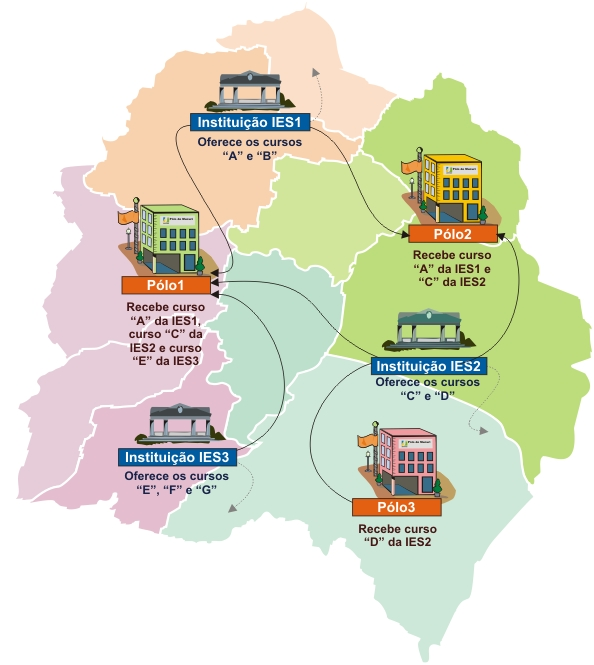
\includegraphics[width=0.35\textwidth]{imagem/cap1/fig1.jpg}}
  \caption{Cen{\' a}rio ilustrando as rela{\c c}{\~ o}es entre os P\'olos e as Institui{\c c}{\~ o}es de Ensino}
  \label{fig:UAB}
 \end{center}
\end{figure}

A Figura~\ref{fig:UAB}, obtida no site da UAB\footnote{\url{http://www.uab.capes.gov.br/}}, 
ilustra bem o funcionamento desta colabora{\c c}{\~ a}o. Nesse cen{\' a}rio, existem três institui{\c c}{\~ o}es
de ensino e três p\'olos. As institui{\c c}{\~ o}es de ensino oferecem alguns cursos para os seus 
p\'olos. Por exemplo, a institui{\c c}{\~ a}o de ensino 1 (IES1) oferece o curso A ao P\'olo 1 e 
o curso B ao p\'olo 2. Como ilustra a figura, diferentes institui{\c c}{\~ o}es de ensino podem
compartilhar a infra-estrutura dos p\'olos para oferecer cursos complementares aos p\'olos.

Como um curso presencial, os cursos {\`a} dist{\^ a}ncia tem uma grade curricular formado 
por um conjunto de disciplinas. Para o aluno se formar, este precisa passar nas disciplinas
exigidas pelo curso. Em uma disciplina de um curso {\`a} dist{\^ a}ncia existem três tipos de docentes:
\begin{itemize}
 \item \textbf{Docentes} -- Os docentes s{\~ a}o educadores que j{\' a} tem experiência no ensino do t\'opico 
 abordado pela disciplina, tendo a ensinado em cursos presenciais ou {\`a} dist{\^ a}ncia. Ele {\'e} o respons{\' a}vel 
 pela disciplina. Al{\'e}m de ter as fun{\c c}{\~ o}es usuais de um professor em uma disciplina presencial, como 
 elaborar provas, 
 o professor em uma disciplina {\`a} dist{\^ a}ncia deve planejar a disciplina, acompanhar os tutores, e montar a sala de aula 
 no Ambiente Virtual de Aprendizado. O professor deve, por exemplo, criar
atividades como f\'oruns, pesquisas de opini{\~ a}o ou tarefas de casa.
 Em alguns cursos tamb{\'e}m {\'e} exigido que o docente visite os p\'olos para ter um contato mais pessoal 
 com os seus alunos e tutores, assim melhorando a intera{\c c}{\~ a}o entre os mesmos.
 
 \item \textbf{Tutores {\`a} Dist{\^ a}ncia} -- Os tutores {\`a} dist{\^ a}ncia, normalmente situados nas institui{\c c}{\~ o}es de ensino, 
 auxiliam os professores no ensino da disciplina. Eles s{\~ a}o respons{\' a}veis por tirar d{\' u}vidas dos alunos e ajud{\' a}-los 
 nos exerc{\' i}cios. Como os tutores tem um contato maior com os alunos, percebendo quais s{\~ a}o as maiores 
 dificuldades dos alunos da disciplina, {\'e} fun{\c c}{\~ a}o dos tutores de comunicar aos professores as suas observa{\c c}{\~ o}es para
 que o professor possa melhor planejar os pr\'oximos passos da disciplina. 
 
 
 \item \textbf{Tutores Presenciais} -- Finalmente, os tutores presenciais s{\~ a}o educadores que est{\~ a}o situados nos p\'olos
 propocionando a rela{\c c}{\~ a}o presencial necess{\' a}ria para um bom aprendizado. 
Al{\'e}m de controlar a frequência dos alunos, os tutores  ajudam os alunos que tem
dificuldades em acessar a sala do curso no 
 \ava, aplicam as provas elaboradas pelos professores nos p\'olos e 
 ajudam os alunos a usarem os recursos dispon{\' i}veis nos $\ava$s. \red{O que mais?}
\end{itemize}

\red{Incluir uma tabela resumindo as responsabilidades dos tutores, professores e alunos}

\section{Diferen{\c c}as ao Ensino Presencial}  Existem muitas diferen{\c c}as entre o ensino presencial e 
o ensino {\`a} dist{\^ a}ncia. Enquanto o contato no ensino presencial entre os educadores e os seus alunos acontece de maneira s{\' i}ncrona, 
quer dizer, em hor{\' a}rios bem definidos, no ensino {\`a} dist{\^ a}ncia, o contato entre os educadores e os seus alunos {\'e} de maneira
ass{\' i}ncrona, quer dizer, pode ocorrer em qualquer momento. Essa diferen{\c c}a faz com que muitas vezes as estrat{\'e}gias de ensino usadas no ensino 
presencial, como o uso de quadro e de slides, n{\~ a}o sejam as mais adequadas no ensino {\`a} dist{\^ a}ncia. O uso de outras ferramentas, 
como f\'oruns e bate-papos, se torna mais importante. Outra diferen{\c c}a {\'e} que o \ead\ exige uma coordena{\c c}{\~ a}o maior entre os professores, tutores
{\`a} dist{\^ a}ncia e tutores presenciais. Como o professor n{\~ a}o tem contato f{\' i}sico com os alunos, ele precisa da avalia{\c c}{\~ a}o dos tutores, 
que tem um contato di{\' a}rio com os alunos, para modelar a sua disciplina e escolher que tipo de atividade que deve ser usada.

De fato, \avas\ s{\~ a}o desenvolvidos com o intuito de incentivar 
a \emph{interatividade} entre alunos, tutores e professores. Esta interatividade {\'e} formentada por ferramentas 
dispon{\' i}veis nos \avas\ como f\'oruns, salas de bate-papo, forma{\c c}{\~ a}o de grupos, realiza{\c c}{\~ a}o de atividades, entre outras. 
Enquanto na aulas presenciais muitos alunos hesitam em participar devido a diversos fatores como timidez, inseguran{\c c}a ou 
mesmo limita{\c c}{\~ o}es de linguagem, muitos alunos tendem a ser mais abertos a discuss{\~ o}es em 
f\'oruns virtuais como evidenciado nas redes sociais como Facebook e Twitter. 

Contudo assim como nas redes sociais, a discuss{\~ a}o num ambiente virtual pode perder o foco e n{\~ a}o atingir 
o seu objetivo final. Portanto tanto para professores como para tutores, {\'e} importante dominar os 
tipos de ferramentas dispon{\' i}veis em um \ava\ para que professores e tutores possam transmitir 
de maneira efetiva o conhecimento da disciplina aos seus alunos.


\section{Ambientes Virtuais de Aprendizado: Moodle}
\label{subsec:cap1:Moodle}

Os Ambientes Virtuais de Aprendizado (\avas) s{\~ a}o plataformas computacionais que rodam ininterruptamente em servidores 
conectados {\`a} Internet. O objetivo de uma \ava\ {\'e} de fornecer os recursos necess{\' a}rios para professores, tutores 
e alunos poderem collaborar a fim de permitir a Educa{\c c}{\~ a}o de Qualidade {\`a} Dist{\^ a}ncia. Um \ava\ permite ao 
professor organizar sua disciplina na forma
de uma p{\' a}gina da Internet. Esta p{\' a}gina pode ser acessada por seus alunos e seus tutores que podem n{\~ a}o somente ver o 
material postado pelo professor, mas tamb{\'e}m pode participar de atividades e interagir entre si atrav{\'e}s, de 
por exemplo, salas de bate-papo. Um \ava\ favorece portanto a cria{\c c}{\~ a}o de uma \emph{comunidade virtual} cujo objetivo 
{\'e} o aprendizado e dissemina{\c c}{\~ a}o do conhecimento.\footnote{No Apêndice~\ref{sec:apendice}, 
descrevemos como alunos dos cursos {\`a} dist{\^ a}ncia da \ufpb\ pode acessar o site do Moodle do instituto.}

Um requisito b{\' a}sico para o uso de um \ava\ {\'e} o conhecimento b{\' a}sico de navega{\c c}{\~ a}o Web. É esperado que um usu{\' a}rio 
saiba acessar uma p{\' a}gina na Internet. 

Por que usar um AVA, por que usar o Moodle?

% \section{Ambiente Virtuais de Aprendizagem}
% 
% Desde o in{\' i}cio dos anos 90 professores ouvem coment{\' a}rios sobre a revolu{\c c}{\~ a}o que vem sendo provocada pela Internet no ensino e na aprendizagem, mas essa revolu{\c c}{\~ a}o ainda n{\~ a}o se materializou. Em lugar disso, um novo conjunto de ferramentas, chamado LMS (Learning Management System em inglês, Sistema de Gest{\~ a}o de Aprendizagem em português), ou AVA como {\'e} mais conhecido (Ambiente Virtual de Aprendizagem), pode ser usado para melhorar seus cursos, tirando proveito das vantagens da Internet sem dispensar a necessidade do professor. Nos {\' u}ltimos dez anos, os AVAs experimentaram um crescimento e amadurecimento r{\' a}pidos e s{\~ a}o, hoje, considerados essenciais em muitas universidades e faculdades.
% 
% 
% 
% \section{Ambientes Virtuais de Aprendizagem}
% 
% AVAs s{\~ a}o aplica{\c c}{\~ o}es Intra/Internet que “rodam” em um servidor web\footnote{Servidor web {\'e} um computador que est{\' a} ligado 7 dias na semana, 24 horas por dia, {\`a} Internet, onde est{\~ a}o gravados os arquivos do Ava e onde est{\' a} um banco de dados que guarda as informa{\c c}{\~ o}es das disciplinas e usu{\' a}rios, podendo ser acessadas mediante autentica{\c c}{\~ a}o, pelos interessados em qualquer lugar onde haja conex{\~ a}o com a rede mundial de computadores.}  e s{\~ a}o acessadas por um navegador (Internet Explorer, Monzila Firefox, Google Chrome, Ópera, Safari, etc.). O servidor est{\' a}, no caso geral, localizado em um departamento ou centro de processamento de uma Universidade, mas pode estar localizado em qualquer lugar do mundo. O professor e os alunos podem acessar o sistema de qualquer lugar onde haja um computador, conex{\~ a}o com a Internet e um navegador Web. Em termos simples, um AVA fornece ao professor ferramentas para que ele crie um curso baseado em uma ambiente Web (site), com controle de acesso de forma tal que somente os alunos do 
curso 
% possam acessar o mesmo. Al{\'e}m deste controle, os AVAs oferecem uma variedade de ferramentas que podem aumentar a efic{\' a}cia de um curso. Pode-se, facilmente, compartilhar materiais de estudo, manter discuss{\~ o}es s{\' i}ncronas e ass{\' i}ncronas\footnote{S{\' i}ncrona: que acontece em tempo real, ao mesmo tempo para todos os participantes. Ass{\' i}ncrona: que n{\~ a}o est{\' a} vinculada ao tempo, ou seja, a discuss{\~ a}o pode ocorrer em per{\' i}odos de tempo distintos, quando uma participa{\c c}{\~ a}o que ocorre agora {\'e} respondida depois e assim por diante.}, aplicar testes de avalia{\c c}{\~ a}o e pesquisas de opini{\~ a}o, coletar e revisar tarefas, al{\'e}m de registrar notas. 
% 
% \index{s{\' i}ncrono}
% \index{ass{\' i}ncrono}
% 
% \section{Recursos AVA}
% \index{Recursos}
% Os ambientes AVAs provêem os mais variados recursos educacionais, no intuito de prover maior did{\' a}tica e eficiência na comunica{\c c}{\~ a}o entre alunos e professores.  Podemos analisar alguns destes recursos a seguir.
% 
% \subsection{Enviando e compartilhando materiais de estudo}
% \index{Materiais de estudo}
% A maioria dos AVAs fornece ferramentas para publicar com facilidade, textos e outros materiais de estudo. Ao inv{\'e}s de usar um editor HTML\footnote{Hypertext Markup Language: Linguagem de Marca{\c c}{\~ a}o para Hipertextos, usada para dar formata{\c c}{\~ a}o {\`a}s p{\' a}ginas web e criar v{\' i}nculos (links) entre elas.} , e ent{\~ a}o, enviar o texto para um servidor Web, usa-se um formul{\' a}rio para publicar conte{\' u}dos (enviar arquivos). Muitos professores costumam publicar em um site da Internet todo o material que produzem e que pode ser {\' u}til para os seus alunos. Por{\'e}m estes ambientes n{\~ a}o possuem tantos recursos did{\' a}ticos como o ambiente AVA.
% 
% 
% \subsection{F\'oruns e Salas de bate-papo}
% 
% \index{F\'oruns e chat}
% 
% Esses recursos fornecem meios de comunica{\c c}{\~ a}o entre o professor e os alunos fora da sala de aula. Os f\'oruns proporcionam mais tempo para reflex{\~ a}o antes que a participa{\c c}{\~ a}o aconte{\c c}a e permitem manter uma discuss{\~ a}o por um per{\' i}odo longo de tempo. As salas de bate-papo, por outro lado, fornecem uma forma de comunica{\c c}{\~ a}o r{\' a}pida e instant{\^ a}nea com professores, tutores e alunos. Podem ser usados para uma discuss{\~ a}o aberta, com tema livre, ou at{\'e} mesmo para uma aula virtual. Sabe-se de um professor que, impedido de falar por motivos m{\'e}dicos, conduz seu curso usando salas de bate-papo para se comunicar com os alunos. Outro uso comum {\'e} aquele feito por grupos de alunos que devem produzir um trabalho e usam o bate-papo online para se organizar e discutir detalhes do trabalho.
% 
% \subsection{Testes e pesquisas de opini{\~ a}o}
% 
% \index{Testes e pesquisas}
% 
% Testes online e pesquisas de opini{\~ a}o podem ser corrigidos e processados instantaneamente. S{\~ a}o grandes ferramentas para 
% permitir que os alunos tenham uma informa{\c c}{\~ a}o r{\' a}pida e eficaz auto-avalia{\c c}{\~ a}o sobre seu desempenho no curso. É comum hoje em dia que editoras e autores de livros texto coloquem question{\' a}rios sobre os cap{\' i}tulos de seus livros em s{\' i}tios na Internet. Podermos citar um exemplo de um professor que conduzindo um curso sobre propaganda na Universidade de S{\~ a}o Francisco (EUA), produz um banco de quest{\~ o}es e adota mini-testes para verificar o progresso dos alunos em seus estudos. A prova final {\'e} um teste com quest{\~ o}es retiradas de todo o banco, de maneira aleat\'oria.
% 
% \subsection{Coletando e revisando tarefas}
% 
% \index{Revis{\~ a}o de tarefas}
% 
% Coletar, corrigir e revisar tarefas (divulgando os resultados da corre{\c c}{\~ a}o com coment{\' a}rios) {\'e} um trabalho cansativo e ma{\c c}ante. Tarefas online {\'e} uma forma f{\' a}cil de coletar e corrigir trabalhos dos alunos e atribuir e divulgar notas. Al{\'e}m disso, pesquisas indicam que o uso de ambientes online com participa{\c c}{\~ a}o anônima, para que os alunos atribuam notas a trabalhos feitos por seus colegas, aumenta a motiva{\c c}{\~ a}o e o desempenho.
% 
% \subsection{Registrando notas}
% 
% \index{Registro de notas}
% 
% Um quadro de notas online permite que os alunos tenham informa{\c c}{\~ o}es sempre atualizadas sobre seu desempenho em um curso. Notas online tamb{\'e}m facilitam cumprir a determina{\c c}{\~ a}o de algumas institui{\c c}{\~ o}es de ensino de que n{\~ a}o tornem p{\' u}blicas as avalia{\c c}{\~ o}es dos alunos. Os quadros de notas dos AVAs permitem, em geral, que os alunos consultem apenas as pr\'oprias notas. É poss{\' i}vel, ainda, copiar o quadro de notas para o computador do professor para processamentos mais elaborados. Embora seja poss{\' i}vel encontrar (ou desenvolver) programas que fa{\c c}am este trabalho, um AVA tem essas ferramentas integradas em seu ambiente. 
% 
% \section{Por que usar um AVA?}
% 
% Aulas têm sido ministradas por milhares de anos sem o uso de computadores ou da Internet. O ambiente em que o professor utiliza um quadro negro, giz e conversa ainda s{\~ a}o ferramentas dominantes no processo educacional. Embora o formato tradicional, ou seja, de forma presencial, possa ainda ser eficaz, o uso das ferramentas acima listadas abrem novas possibilidades de aprendizagem que n{\~ a}o eram imagin{\' a}veis h{\' a} anos atr{\' a}s.
% 
% No momento, uma grande quantidade de pesquisa ainda {\'e} feita sobre como combinar aprendizagem presencial com os chamados cursos h{\' i}bridos. Que s{\~ a}o os cursos que combinam aulas presenciais e aula {\`a} dist{\^ a}ncia. Imagine transferir a maior parte do material did{\' a}tico de seu curso para um ambiente virtual e aproveitar seu tempo em aula para discuss{\~ o}es, quest{\~ o}es e resolu{\c c}{\~ a}o de problemas. Muitos professores j{\' a} descobriram que eles podem economizar tempo e melhorar a aprendizagem de seus alunos comportando-se dessa maneira. Isto permite que os alunos usem os encontros presencias para a solu{\c c}{\~ a}o de problemas e os professores possam transformar suas aulas em palestras de contextualiza{\c c}{\~ a}o, abandonando a preocupa{\c c}{\~ a}o de ter que cumprir o programa de forma presencial.
% 
% As discuss{\~ o}es online permitem que muitos alunos se expressem em formas que eles n{\~ a}o conseguiriam em aulas regulares. Muitos deles relutam em falar em aula por motivos variados: timidez, inseguran{\c c}a, ou mesmo limita{\c c}{\~ o}es de linguagem. A possibilidade de criar um ambiente de constru{\c c}{\~ a}o coletiva do conhecimento online {\'e}, muitas vezes, de grande import{\^ a}ncia para alguns alunos. Muitos professores relatam um aumento significativo na participa{\c c}{\~ a}o quando se introduz esse formato de aprendizagem. H{\' a} outro n{\' u}mero de raz{\~ o}es para se pensar na utiliza{\c c}{\~ a}o de ambientes virtuais em seus cursos, como por exemplo:
% 
% \begin{itemize}
%  \item Demanda dos alunos: os alunos (especialmente os de curso superior) têm, hoje, um grau de inclus{\~ a}o digital muito maior, e utilizam muitos sistemas de comunica{\c c}{\~ a}o como (MSN, Facebook, GTalk, Skype, por exemplo) eles se sentem {\`a} vontade em um AVA;
%  \item Hor{\' a}rios dos alunos: aumenta cada vez mais o n{\' u}mero de alunos que trabalha. Em alguns pa{\' i}ses, a m{\'e}dia semanal de trabalho dos alunos de cursos superiores chega a 20 horas. Com ambientes online eles podem adequar seus hor{\' a}rios de trabalho {\`a}s atividades de um curso;
%  \item Cursos melhores: se bem usado, um AVA pode tornar suas aulas mais eficazes e melhores. Movendo parte de seu curso para a Internet {\'e} poss{\' i}vel aproveitar os encontros presenciais para envolver os alunos em quest{\~ o}es b{\' a}sicas do curso e convid{\' a}-lo a refletir sobre temas correlatos. O professor pode, tamb{\'e}m, aproveitar o tempo discorrendo sobre temas que sempre desejou abordar e foi impedido pelo fato de ter que cumprir o programa.
% \end{itemize}
% 
% Você provavelmente ouviu os argumentos at{\'e} aqui apresentados durante a {\' u}ltima d{\'e}cada do s{\'e}culo XX. Ent{\~ a}o, o que mudou? Hoje, os AVAs est{\~ a}o melhores estruturados, mais maduros, e f{\' a}ceis de usar do que foram h{\' a} alguns anos atr{\' a}s. A tecnologia que envolve a disponibilidade deste ambiente tornou-se melhor e mais est{\' a}vel. H{\' a} pouco tempo, muitos sistemas eram projetados para uso pessoal, ou para uso de um grupo espec{\' i}fico de pessoas, e eram comercializados na forma original, mostrando-se pouco flex{\' i}veis. Dois dos sistemas mais conhecidos (Blackboard e WebCT) come{\c c}aram como projetos para pequenas faculdades e se tornaram l{\' i}deres do mercado.
% 
% Entretanto, liderar o mercado n{\~ a}o significa ser o melhor ou mais bem projetado. De fato, os l{\' i}deres de mercado têm tido dificuldades para manter seu crescimento e argumenta-se inclusive que o esfor{\c c}o para manter essa lideran{\c c}a tem prejudicado a qualidade final do produto.
% 
% 
% 
% \section{Por que o Moodle {\'e} diferente?}
% 
% Muitos administradores de ambientes de aprendizagem têm declarado sua ades{\~ a}o ao Moodle principalmente em virtude de ser ele um sistema aberto baseado em uma forte filosofia educacional com uma comunidade de usu{\' a}rios que cresce dia a dia e contribui para o desenvolvimento e apoio a novos usu{\' a}rios. A seguir podem-se analisar detalhadamente algumas vantagens do AVA Moodle.
% 
% \section{Gratuito e de fonte aberta (c\'odigo aberto)}
% 
% A express{\~ a}o fonte aberta (do inglês open source) tornou-se um termo restrito a certo c{\' i}rculo de pessoas. Para aqueles que n{\~ a}o est{\~ a}o acostumados com a linguagem t{\'e}cnica {\'e} dif{\' i}cil entender como essa id{\'e}ia estranha e poderosa mudou para sempre o mundo do desenvolvimento de programas para computador. A id{\'e}ia em si {\'e} bastante simples: fonte aberta significa que os usu{\' a}rios têm acesso ao c\'odigo fonte do programa. Pode-se examinar (alterar, ampliar, modificar) o programa ou mesmo usar partes dele para aplica{\c c}{\~ o}es de interesse pessoal.
% 
% Programas para computador de fonte aberta adotam valores acadêmicos de liberdade, avalia{\c c}{\~ a}o pelos pares e compartilhamento do conhecimento. Qualquer pessoa pode baixar o Moodle gratuitamente, modificar ou acrescentar m\'odulos, corrigir erros, melhorar seu desempenho ou simplesmente aprender observando como outras pessoas usam o ambiente e resolvem problemas. Alem disso, ao contr{\' a}rio dos sistemas propriet{\' a}rios, o Moodle pode ser instalado sem nenhum custo (em quantos servidores você desejar). Ningu{\'e}m poder{\' a} retir{\' a}-lo de você, aumentar os custos de manuten{\c c}{\~ a}o ou fazê-lo pagar por atualiza{\c c}{\~ o}es. Ningu{\'e}m pode for{\c c}{\' a}-lo a fazer atualiza{\c c}{\~ o}es, comprar ferramentas que você n{\~ a}o deseja ou determinar quantos usu{\' a}rios você pode ter.
% 
% 
% \section{Pedagogia}
% 
% O criador do Moodle, Martin Dougiamas, tem forma{\c c}{\~ a}o em educa{\c c}{\~ a}o e inform{\' a}tica. Isto o conduziu a adotar o Construcionismo Social como a estrutura pedag\'ogica em que est{\' a} baseado o ambiente. Isto {\'e} inovador uma vez que os ambientes de gest{\~ a}o de aprendizagem s{\~ a}o, em geral, constru{\' i}dos em torno de ferramentas computacionais. Pode-se afirmar que os AVAs comerciais s{\~ a}o voltados para ferramentas enquanto o Moodle {\'e} voltado para aprendizagem. O Construcionismo Social baseia-se na id{\'e}ia de que pessoas aprendem melhor quando engajadas em um processo social de constru{\c c}{\~ a}o do conhecimento, pelo ato de construir alguma coisa para outros. Este {\'e} um conceito um tanto sint{\'e}tico que pode ser mais bem detalhado. O termo processo social sugere que a aprendizagem {\'e} alguma coisa que se faz em grupos. Deste ponto de vista, aprendizagem {\'e} um processo de negocia{\c c}{\~ a}o de significados em uma cultura de s{\' i}mbolos e artefatos compartilhados. O processo de negocia{\c c}{\~ a}o de significados e utiliza{\c c}{\~ a}o de recursos compartilhados {\'e} o processo de 
% constru{\c c}{\~ a}o do conhecimento. N\'os n{\~ a}o somos um quadro branco quando entramos no processo de aprendizagem. N\'os precisamos testar nossos novos conhecimentos comparando-os com velhas cren{\c c}as e incorporando-os em nossas estruturas de conhecimento j{\' a} existentes. Parte do processo de teste e negocia{\c c}{\~ a}o envolve a cria{\c c}{\~ a}o de artefatos e s{\' i}mbolos para que outros interajam com eles.
% 
% E como isto tem rela{\c c}{\~ a}o com o ambiente Moodle? A primeira indica{\c c}{\~ a}o est{\' a} na interface. Enquanto AVAs centrados em ferramentas fornecem uma lista de ferramentas como sendo a interface, o ambiente Moodle coloca as ferramentas em uma interface que faz da aprendizagem a tarefa central. Pode-se estruturar um curso no ambiente Moodle nos formatos semanal, t\'opicos ou social. Al{\'e}m disso, enquanto outros AVAs se estruturam em um modelo de conte{\' u}do que encoraja os professores a carregar uma infinidade de conte{\' u}dos est{\' a}ticos, o ambiente Moodle enfoca o trabalho em ferramentas para discuss{\~ a}o e compartilhamento de experiências. Assim, a ênfase est{\' a} n{\~ a}o em distribuir informa{\c c}{\~ a}o, mas em compartilhar id{\'e}ias e engajar os alunos na constru{\c c}{\~ a}o do conhecimento.
% 
% A filosofia de projeto do Moodle torna-o um pacote amig{\' a}vel para professores e representa a primeira gera{\c c}{\~ a}o de ferramentas educacionais realmente {\' u}teis.
% 
% O Moodle tem uma comunidade de usu{\' a}rios grande e com participa{\c c}{\~ a}o na manuten{\c c}{\~ a}o da distribui{\c c}{\~ a}o, sugerindo sempre modifica{\c c}{\~ o}es, novas habilidades e reportando eventuais defeitos. Pode-se acessar a comunidade em  \url{http://moodle.org/}(em inglês) e no ambiente de discuss{\~ a}o do Moodle Brasileiro em \url{http://moodle.org/?lang=pt_br em português}.
% 
% A comunidade Moodle tem sido indispens{\' a}vel para o sucesso do sistema. Com tantos usu{\' a}rios em todo o mundo sempre h{\' a} algu{\'e}m que pode responder a perguntas e dar conselhos. Ao mesmo tempo, os desenvolvedores e usu{\' a}rios do Moodle trabalham juntos para garantir qualidade, adicionar novos m\'odulos e ferramentas e sugerir novas id{\'e}ias de desenvolvimento do ambiente. Martin Dougiamas e sua equipe s{\~ a}o respons{\' a}veis pela decis{\~ a}o de aceitar ou n{\~ a}o as sugest{\~ o}es dos colaboradores. Em virtude do fato do ambiente ser de fonte aberta muitas pessoas desenvolvem novos m\'odulos e os submetem {\`a} aprecia{\c c}{\~ a}o dos desenvolvedores e da comunidade. Isto funciona como um grande departamento de desenvolvimento e controle de qualidade.
% 
% Essas três vantagens - fonte aberta, Construcionismo Social e comunidade de desenvolvimento - fazem do Moodle um espa{\c c}o de aprendizagem {\' u}nico no mundo.
% 
%                                                      \begin{flushright}Adapta{\c c}{\~ a}o do texto do prof. Athail Rangel Pulino Filho
%                                                       
%                                                                                  Universidade de Bras{\' i}lia, DF\end{flushright} 
%                                                                                  

